\documentclass[10pt,twocolumn,letterpaper]{article}

\usepackage{cvpr}
\usepackage{times}
\usepackage{epsfig}
\usepackage{graphicx}
\usepackage{amsmath}
\usepackage{amssymb}

% Include other packages here, before hyperref.

% If you comment hyperref and then uncomment it, you should delete
% egpaper.aux before re-running latex.  (Or just hit 'q' on the first latex
% run, let it finish, and you should be clear).
\usepackage[breaklinks=true,bookmarks=false]{hyperref}

% \cvprfinalcopy % *** Uncomment this line for the final submission

\def\cvprPaperID{****} % *** Enter the CVPR Paper ID here
\def\httilde{\mbox{\tt\raisebox{-.5ex}{\symbol{126}}}}

% Pages are numbered in submission mode, and unnumbered in camera-ready
%\ifcvprfinal\pagestyle{empty}\fi
\setcounter{page}{1}
\begin{document}

%%%%%%%%% TITLE
\title{Comparing Fixed-weight and Bayesian Neural networks for 3D Object Detection in the context of Autonomous Driving}

\author{
Jaswanth Bandlamudi\\
{Hochschule Bonn-Rhein sieg\\
 jaswanth.bandlamudi@smail.inf.h-brs.de}
\and 
Octavio Arriaga\\
{DFKI, Bremen\\
 arriagac@uni-bremen.de}
\and
Paul G Pl\"{o}ger\\
{Hochschule Bonn-Rhein sieg\\
 paul.pl\"{o}ger@h-brs.de}
\and
Anastassia K\"{u}stenmacher\\
{Hochschule Bonn-Rhein sieg\\
 anastassia.k\"{u}stenmacher@h-brs.de}

}

\maketitle
%\thispagestyle{empty}

%%%%%%%%% ABSTRACT
\begin{abstract}
    Accurate perception and understanding of a scene is required for the safe operation of autonomous agents. Current state-of-the-art methods use Deep Neural Networks (DNN) in order to localize and classify objects. However, these neural networks are often point estimates which have been reported to provide overconfident results [?]. This may lead to catastrophic failures; specifically, in critical tasks such as autonomous driving. On the other hand, Bayesian Neural Networks (BNNs) can provide an extra measure of uncertainty along with the object proposals. Thus, in this work we compare the performances of fixed-weight Neural Networks versus BNNs on the task of localization and classification of objects in 3D space. Our results show that fixed-weight neural networks are indeed over-confident in 3D detection task, while BNNs do provide us with a better uncertainty estimation, while still retaining the same accuracy [?].
\end{abstract}

%-------------------------------------------------------------------------
%%%%%%%%% BODY TEXT
\section{Introduction}

In order to properly perceive the environment, autonomous cars must be able to reliable solve tasks such as lane detection, vehicle detection, and Vulnerable Road Users (VRU)\footnote{Vulnerable Road Users (VRU) are defined in the European Union Intelligent Transportation Systems Directive as "non-motorized road users, such as pedestrians and cyclists as well as motorcyclists and persons with disabilities or reduced mobility and orientation".} detection. Thus, autonomous cars require that the vehicle's perception module predicts the 3D position of the agents\footnote{Agents in this work refers to a car, pedestrians, and cyclist present in the operating environment} around~\cite{KITTI2012}. This task has to be carried out with high accuracy and should be robust against adverse weather, occlusions and extreme lighting conditions. 

The task of object detection is carried out with the usage of Deep Neural Networks(DNNs) \cite{Rao2018, Arnold2019} that use RGB cameras \cite{Chen2016, Mousavian2017, Chabot2017, Chen2017}, LiDAR \cite{VOTE3DEEP2017, Zhou2018, Sahba2019, Simon2018, Xiang2015} or a fusion of both \cite{Du2018, FPointnet2018, AVOD2018, FrustumConvnet2019}. Furthermore, advances in this research have been possible by datasets such as KITTI \cite{KITTI2012}, Waymo\cite{Waymo2019}, nuTonomy\cite{Caesar2020}.

However, there are failures for using DNNs in safety-related tasks. For example, \label{GoogleFailure} the image-classification model by Google had wrongly classified photos of some humans as gorillas \cite{Mulshine2015}. Another such failure was reported\label{Uberfailure} when a self-driving car from Uber hit a jay-walking pedestrian and resulted in death \cite{SLJCW2018}. Both of these examples show that DNNs are prone to failures. 

DNNs have out-performed the conventional statistical approaches in both accuracy and generalizability. However, they cannot alone quantify the uncertainty in the outputs. The classification models provide predictive probabilities which are softmax outputs of a model. But the softmax probabilities are wrongfully interpreted as an uncertainty metric. This leads to false positives with very high scores \cite{Blundell2015, Malinin2018}. This sort of behavior is unsolicited in applications like autonomous driving, making these methods incompatible with safety-critical applications. 

BNNs \cite{tran2016edward, Shridhar2018, Tran2019} are a class of neural networks in which the weights are initialized as a distribution $p(w)$, and training includes obtaining a posterior distribution over weights represented by $p (w|D)$, where $D$ is the dataset on which the model is trained. $p (w|D)$ captures the model uncertainty. Additionally, BNNs also permit the knowledge of uncertainty source \cite{Henne2020}. The predictive uncertainty is classified into epistemic uncertainty and aleatoric uncertainty \cite{Kendall2017}. Aleatoric uncertainty is further classified into Homoscedastic uncertainty, which stays constant for different inputs and Heteroscedastic uncertainty varies with input, and some being more affected because of the noise from the environment.


\subsection{Contributions}
In this work, we develop a Flipout-based Bayesian neural network \cite{Wen2018} architecture to capture the uncertainty of a Frustum-PointNet for 3D object detection. The main contributions of this paper are: 
\begin{itemize}
    \item We successfully combined BNNs and Frustum-PointNets for 3D object detection 
    \item We obtain slightly better results using our Bayesian model versus the fixed-weight architecture
    \item We provide a quantiative and a qualitative depiction of uncertainty.
\end{itemize}
    
    Along with the above elements we also provide a literature review of the 3D object detection methods and the uncertainty quantification techniques used in BNNs.
%-------------------------------------------------------------------------
\section{Related Work}
In this section, we summarize various 3D object detection methods, as well as different BNN architectures for extracting uncertainty using the chosen 3D object detection network.

\subsection{3D object detection in Autonomous Driving}
The main aim of the 3D object detection model is to process information from sensors like Light Detection and Ranging (LiDAR), cameras, Radio Detection and Ranging (RADAR), and output a 3D bounding box along with class labels of the agents in the perceived environment. It is also referred to as amodal 3D object detection \cite{Arnold2019}, which means the model should fit a 3D bounding box for the whole object even though only a part of it is visible.

% \subsubsection{LiDAR Point Cloud based 3D Object Detection}
% This category of 3D object detection networks aims to represent point clouds similar to images, so that the mature CNN-based object detection models can be used to regress the necessary dimensions. There are two methods in this category which are volumetric grid-based (Voxel-based) and projection maps based.

% Vote3D \cite{VOTE3DEEP2017} uses voting in order to determine if a cell is occupied or not. For detection purposes, a search in the voxel space is performed and for classification, a linear Support Vector Machine (SVM) is used. Vote3Deep is another method that extends on Vote3D by processing the whole point cloud using a neural network and fixed class sizes are used based on the classification output. Voxelnet \cite{Zhou2018} consists of three stages a voxel feature extraction layer which is a modified PointNet \cite{Pointnet2017} and outputs a sparse 4D voxel-wise feature vector of pre-defined size. These outputs are fed into 3D convolution layers which results in a 3D feature map and the output is processed by a Region Proposal Network (RPN). The outputs of RPN are the confidence scores and the 3D box anchors. \textit{Li et al.} \cite{Li2017} used a LiDAR projection which encodes the point clouds distance from the ground and the range of the points. This map is processed using a 2D FCN to downsample the provided map and then up samples to regress objectness, which defines whether the point is a vehicle part or not and bounding box predictions and also represents the 3D bounding box edges. Complexer-YOLO \cite{Simon2018} proposed by \textit{Simon et al.}, uses a BEV projection of the point cloud and uses a modified Fast-RCNN model as the backbone in order to regress the 3D bounding box details. This method has achieved a benchmark 50 fps processing speed but with a deteriorated orientation angle accuracy.

% \subsubsection{Sensor Fusion based 3D Object Detection}
The best-performing methods for 3D object detection are majorly fusion-based, as reported by KITTI Benchmark tests \cite{KITTI2012}. This results are possible by the dense input provided by the camera and the depth information provided by the LiDAR point cloud. The combination of these orthogonal data sources provides features to predict the depth of the objects as well as its semantics.

In the work reported by \textit{Du et al.} \cite{Du2018}, a pre-trained 2D detection network proposes a candidate for a bounding box. This information is fused with the 3D features from the point cloud, in order to regress the 3D parameters. ?????? MV3D \cite{MV3D2017} by \textit{Chen et al.}, in which three inputs RGB image, point cloud projected onto the front view, and BEV point cloud are consumed. The front view projection provides information about height, intensity, and distance and the BEV images hold density, intensity, and height information. Then an RPN generates 3D object proposals from BEV only and these proposals are projected to multiple views. AVOD is proposed by \textit{Ku et al.} \cite{AVOD2018}, a deep continuous fusion paradigm is utilized where a 2D BEV projection map is fed to a CNN and another CNN extracts feature maps from the monocular image. These features are fed to a parallel network, which consists of an RPN and a detection network. Frustum-PointNet proposed by \textit{Qi et al.} \cite{FPointnet2018}, where a 2D object detector is used to generate a detection in 2D and this 2D detection is used to reduce the search space to process only the required part of the point cloud where the object presence is given. The frustum generated is fed to an encoder-decoder-based instance segmentation network which assigns the labels to the points in the point cloud based on the class label. This helps in finding the objects when there is a presence of partial occlusion. The segmented point cloud is passed to a PointNet \cite{Pointnet2017} based amodal bounding box estimation which regresses the 3D bounding boxes.

\subsection{Bayesian Neural Networks}
In conventional DNNs, weights are modeled as point estimates. These point estimates resulted in the network being deterministic for provided inputs. Whereas, Bayesian Neural Networks (BNNs) models the weights as a distribution of weights defined over the given dataset $D$. This helps in extracting uncertainty by sampling weights from the posterior distribution of weights.

Let us consider a dataset $D=\left\{\left(x^{(1)}, y^{(1)}\right),\left(x^{(2)}, y^{(2)}\right), \ldots,\left(x^{(N)}, y^{(N)}\right)\right\}$, and $w$ be the weights of the neural network that are to be learnt from the dataset $D$ provided. The posterior distribution $p(w \mid D)$ is obtained by applying Bayes rule as in Equation \ref{Training_Bayes_Rule}
    \begin{equation}
        \label{Training_Bayes_Rule}
        p(w \mid D)=\frac{p(D \mid w) p(w)}{p(D)}
    \end{equation}
Calculating the denominator $p(D)$ is not possible because of the integration over all the weights. The DNNs generally have millions of weights and integrating all over them is computationally expensive. Hence, we approximate the $p(w \mid D)$ distribution.

\textit{Graves et al,} \cite{Graves2011} proposed that the posterior distribution $p(w \mid D)$ can be approximated to be a parameterized distribution $q(w)$ and optimize those distributions over the weight parameters to obtain the best approximation.
        
The approximation is judged using Kullback-Leibler (KL) divergence \cite{Kullback1959} as shown in Equation \ref{KL-D}.
    \begin{equation}
        \label{KL-D}
        \begin{aligned}
            \mathrm{KL}(q(w) \| p(w \mid D)) &=\operatorname{KL}(q(w) \| p(w))+\log p(D)\\ -\mathbb{E}_{q(w)}[\log p(D \mid w)]
        \end{aligned}
    \end{equation}

Hence, VI poses the problem of finding the $p(w \mid D)$ into a maximizing ELBO problem. Once the optimization problem is defined we can use Bayes by backprop by \textit{Shridhar et al.} \cite{shridhar2018uncertainty}, to extract the best approximation of posterior which maximizes the ELBO. Bayes by Back-propagation was first introduced by \textit{Blundell et al.} \cite{Blundell2015}, which allowed the usage of current back-propagation algorithm work by replacing the weights with a parameterized distribution. Hence, the optimal parameters $\theta^{opt}$ which consists of respective mean and variance ($\mu, \sigma$) are defined as  
        
\begin{equation}
\label{optim_param}
    \begin{aligned}
    \theta^{opt} =\operatorname{argmin}_{\theta} \mathbf{K L}[q(\mathbf{w} \mid \theta) \| P(\mathbf{w})]- \\ \mathbb{E}_{q(\mathbf{w} \mid \theta)}[\log P(\mathfrak{D} \mid \mathbf{w})]
    \end{aligned}
\end{equation}

% Let us consider, $$f(w,\theta) = \log \frac{q(\mathbf{w} \mid \theta)}{P(\mathbf{w}) P(\mathfrak{D} \mid \mathbf{w})}$$,  $$\implies f(\mathbf{w}, \theta)  \approx \sum_{i=1}^{n} \log q\left(\mathbf{w}^{(i)} \mid \theta\right)-\\ \log P\left(\mathbf{w}^{(i)}\right)-\log P\left(\mathfrak{D} \mid \mathbf{w}^{(i)}\right)$$, in which $w^{i}$ are the samples drawn from the variational posterior $q(w)$.
        
Substituting this in Equation \ref{optim_param} we get, 
\begin{equation}
    \theta^{*}=\operatorname{argmin}_{\theta}\newline \mathbb{E}_{q(\mathbf{w} \mid \theta)} f(\mathbf{w}, \theta)
\end{equation}

But, the above objective function cannot be used with a standard back-propagation algorithm. This is due to the inability to achieve differentiation of the stochastic node inside the objective function. Hence, \textit{Kingma et al} \cite{Kingma2015} proposed a reparameterization trick by representing the stochastic node as a point value parameterized by a distribution from which a scale value for the weights can be sampled from. This resulted in gradient calculation through general back-propagation. 

In case of CNNs, \textit{Shridhar et al.} proposed to sample layer activations instead of weights, this results in a estimated posterior distribution $q_{\theta}\left(\theta_{\mathrm{i} j h w} \mid D a t a\right)$.The resultant equation for sampling the activation is written as 
        
\begin{equation}b_{j}=A_{\mathrm{i}} * \mu_{\mathrm{i}}+\varepsilon_{j} \cdot \sqrt{A_{\mathrm{i}}^{2} *\left(\alpha_{\mathrm{i}} \cdot \mu_{\mathrm{i}}^{2}\right)}\end{equation}

$b$ is the layer activation, $\varepsilon_{j} \epsilon N(0,1)$, $ A $ is the receptive field area.

\textit{Flipout based Weight-sampling methods:}
Though the reparameterization method is able to achieve a VI approximation $q(w)$ by backpropogation. But the resultant weight updates in batch are correlated resulting in updates with high variance. Flipout is introduced in \textit{Wen et al.} aims to decorrelate the gradients between every sample. This work achieved by making the following assumptions:
\begin{enumerate}
 \item The sampling of different weights is independent of each other. 
 \item The posterior distribution is symmetric around 0. 
\end{enumerate}

Flipout suggests using a posterior distribution ($q_{\theta}$) which is jointly used by every weight sample on the mini-batch, and an element-wise multiplication is performed by another rank-one sign matrix for every sample. A random sign matrix $E$ which is independent of posterior distribution $q_{\theta}$. The weight sampling is done by multiplying $E$ and the posterior distribution $$W = q_{\theta}, E$$.

With the availability of the approximation $q(w)$ of $p(w \mid D)$ obtained using the VI method we can infer an output $y^{*}$ for any given input $x^{*}$ by integrating over the weights available as shown in Equation \ref{final_inference}.

\begin{equation}
    \label{final_inference}
    p\left(y^{*} \mid x^{*}, D\right) \approx \frac{1}{K} \sum_{k=1}^{K} p\left(y^{*} \mid x^{*}, w^{k}\right)
\end{equation}
    
        
% \subsection{Ensemble Networks}
% In this section we introduce Ensemble method for uncertainty quantification in which we use multiple checkpoints in a single training run. 
% \subsubsection{Sub-ensemble networks}
% In this section we introduce Sub-ensemble method for uncertainty quantification in which we use multiple models with different number of trainable layers leading to models with different weight values and use ti for uncertainty evaluation. 
% %-------------------------------------------------------------------------
% % Can be removed
% % \section{Frustum-PointNet architecture}
% % Should I keep this section ?
% % \subsection{Frustum Extraction}
% % \subsection{Instance segmentation}
% % \subsection{Spatial-Transformer Network}
% % \subsection{Bounding-Box Network}
% % \subsection{Loss function}
% %-------------------------------------------------------------------------
\section{Uncertainty Quantification}
In this section, we will summarize the method used to quantify the uncertainty in 3D object detection.
\subsection{Quantifying Epistemic Uncertainty in Agent Classification}
        \label{uncertainty in classification}
        Uncertainty in classification can be quantified using the Shannon entropy of the final softmax scores in Equation \ref{Classification Uncertainty Equation}. As used by \textit{Feng et al.} \cite{Feng2018}, for an input of $x^{*}$, the classification probability of class for N with the availability of the probability score is calculated using Equation \ref{prob_calc}. This probability is used to calculate Shannon entropy (SE).

        \begin{equation}
            \label{prob_calc}
            \begin{aligned}
                p\left(c \mid \mathbf{x}^{*}\right) &=\mathbb{E}_{p(\mathbf{W} \mid \mathbf{X}, \mathbf{Y})} p\left(c \mid \mathbf{x}^{*}, \mathbf{W}\right) \\
                & \approx \frac{1}{N} \sum_{i=1}^{N} s_{\mathbf{x}^{*}}^{i}
            \end{aligned}
        \end{equation}
        
        \begin{equation}
            \label{Classification Uncertainty Equation}
            \begin{array}{l}
                S E\left(\mathbf{y}^{*} \mid \mathbf{x}^{*}\right)=\mathbb{H}\left(\mathbf{y}^{*} \mid \mathbf{x}^{*}\right) \\
                =-p\left(c \mid \mathbf{x}^{*}\right) \log p\left(c \mid \mathbf{x}^{*}\right)-p\left(\neg c \mid \mathbf{x}^{*}\right) \log p\left(\neg c \mid \mathbf{x}^{*}\right) \\
                \approx-\frac{1}{N} \sum_{i=1}^{N} s_{\mathbf{x}}^{i} \cdot \log \frac{1}{N} \sum_{i=1}^{N} s_{\mathbf{x}^{*}}^{i}- \\ \left(1-\frac{1}{N} \sum_{i=1}^{N} s_{\mathbf{x}^{*}}^{i}\right) \log \left(1-\frac{1}{N} \sum_{i=1}^{N} s_{\mathbf{x}^{*}}^{i}\right)
            \end{array}
        \end{equation}
        
        If the SE value is zero, then the network is most certain of the output and when the SE value is higher the network is not certain of the classification result.
        
         \subsection{Quantifying Total-Uncertainty in Regression}
         \label{uncertainty in bounding box regression}
         To find the spatial uncertainty in the bounding box parameters \textit{Feng et al.} \cite{Feng2018} proposed to calculate Total Variance (TV), which represents how much each measurement varies from their mean value.
         
         \begin{enumerate}
             \item Transform the bounding box detections into world reference frame and the mean value of the detections regressed during N forward passes is calculated.
             \item Covariance matrix of the detections is calculated using the following the equation $C\left(\mathbf{x}^{*}\right)=\frac{1}{N} \sum_{i=1}^{N} \hat{\mathbf{v}}_{\mathbf{x}^{*}}^{i} \hat{\mathbf{v}}_{\mathbf{x}^{*}}^{i^{T}}-\mathbf{I}_{\mathbf{x}^{*}} \mathbf{I}_{\mathbf{x}^{*}}^{T}$.
             \item Total variance is calculating by taking the trace of the covariance matric $C(x^{*})$.
         \end{enumerate}
         
         The Total variance spans from $[0,+\infty)$, the higher the value represents the higher the epistemic uncertainty in regressed bounding box parameters.
%-------------------------------------------------------------------------
\section{Experimental Results}
\subsection{Training Frustum-PointNet }
The main aim of this experiment is to train a  Frustum-PointNet using Lyft dataset. The model is trained using a total of 230,944 samples divided into 7,217 training samples of batch size 32. The training is done for 178 (i,e. Three days) epochs.
% \begin{figure}[h]
% 	\begin{subfigure}[t]{0.2\textwidth}
% 		\centering
% 		\includegraphics[width=\textwidth]{images/LYFT_Detections/car_detection_3d.pdf}
% 	\end{subfigure}
%     \hspace{1cm}
%     \vspace{0.5cm}
% 	\begin{subfigure}[t]{0.2\textwidth}
% 		\centering
% 		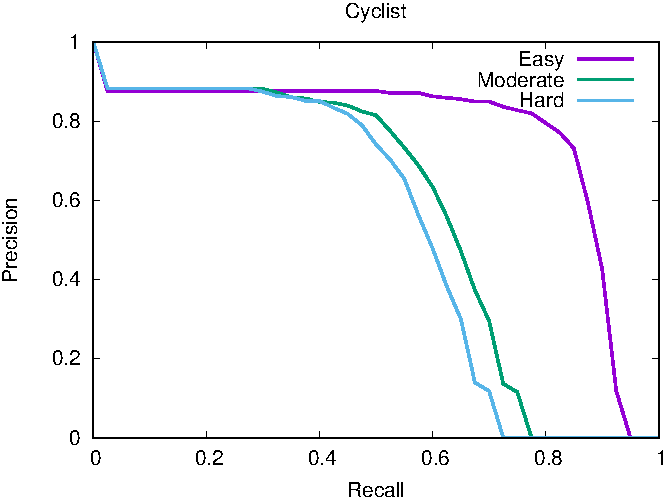
\includegraphics[width=\textwidth]{images/LYFT_Detections/cyclist_detection_3d.PDF}
% 	\end{subfigure}
% 	\hspace{1cm}
% 	\vspace{0.5cm}
% 	\begin{subfigure}[t]{0.2\textwidth}
% 		\centering
% 		\includegraphics[width=\textwidth]{images/LYFT_Detections/pedestrian_detection_3d.PDF}
% 	\end{subfigure}
%     	\caption[Precision-Recall graphs from Lyft 3D detection evaluation]{Precision-Recall graphs from Lyft 3D detection evaluation}
%     	\label{fig:PR-graphs-1}
% \end{figure}

% \begin{figure}[!htbp]
%         \centering
% 		\includegraphics[scale = 0.4]{images/LYFT_Detections/car_detection_3d.pdf}
%         \caption[Extracted frustum point cloud after Normalization]{Precision-Recall graphs for Car detection}
%         \label{fig:Norm Point Cloud}
% \end{figure}
% \begin{figure}[!htbp]
%         \centering
% 		\includegraphics[scale= 0.4]{latex/images/LYFT_Detections/cyclist_detection_3d.pdf}
%         \caption[Extracted frustum point cloud after Normalization]{Precision-Recall graphs for Cyclist detection}
%         \label{fig:Norm Point Cloud}
% \end{figure}
% \begin{figure}[!htbp]
%         \centering
% 		\includegraphics[scale = 0.4]{latex/images/LYFT_Detections/pedestrian_detection_3d.pdf}
%         \caption[Extracted frustum point cloud after Normalization]{Precision-Recall graphs for Pedestrian detection}
%         \label{fig:Norm Point Cloud}
% \end{figure}
\begin{table}[!htbp]
    \caption[3D AP calculated for 2D proposals generated from 3D Annotations]{3D Average Precision values for 3D object detection on Lyft dataset \label{3DAP Values-1} \cite{Lyft2019}}
    \centering
    \begin{tabular}{|c|c|c|c|}
        \hline \textbf{Difficulty} & \textbf{Car (\%)} & \textbf{Cyclist (\%)} & \textbf{Pedestrian (\%)}  \\
        \hline \textbf{Easy} & 80.19  & 69.79  & 60.59 \\
        \hline \textbf{Moderate} & 64.74  & 42.35 & 34.93 \\
        \hline \textbf{Hard} & 58.28  & 37.28  & 34.93  \\
        \hline
    \end{tabular}
    \end{table}
\subsection{Bayesian Neural network modelling and evaluation}
We converted the Frustum-PointNet model into a Bayesian model using TensorFlow probability library \cite{Tran2019}. But, we observed that the model is under-fitting. We converted the Frustum-PointNet model into partial-Bayesian model, by fixing the weights of instance segmentation model and converting the spatial-transformer network and bounding box network into Bayesian model which fitted during training.
% \begin{figure}[!htbp]
%         \centering
% 		\includegraphics[scale = 0.4]{latex/images/Part-Bayesian F_Pointnet_Results/car_detection_3d.pdf}
%         \caption[Extracted frustum point cloud after Normalization]{Precision-Recall graphs for Car detection}
%         \label{fig:Norm Point Cloud}
% \end{figure}
% \begin{figure}[!htbp]
%         \centering
% 		\includegraphics[scale = 0.4]{latex/images/Part-Bayesian F_Pointnet_Results/cyclist_detection_3d.pdf}
%         \caption[Extracted frustum point cloud after Normalization]{Precision-Recall graphs for Cyclist detection}
%         \label{fig:Norm Point Cloud}
% \end{figure}
% \begin{figure}[!htbp]
%         \centering
% 		\includegraphics[scale = 0.4]{latex/images/Part-Bayesian F_Pointnet_Results/pedestrian_detection_3d.pdf}
%         \caption[Extracted frustum point cloud after Normalization]{Precision-Recall graphs for Pedestrian detection}
%         \label{fig:Norm Point Cloud}
% \end{figure}
\begin{table}[!htbp]
    \caption[3D AP calculated for 2D proposals generated from 3D Annotations]{3D Average Precision values for 3D object detection on Lyft dataset \label{3DAP Values-1} \cite{Lyft2019}}
    \centering
    \begin{tabular}{|c|c|c|c|}
        \hline \textbf{Difficulty} & \textbf{Car (\%)} & \textbf{Cyclist (\%)} & \textbf{Pedestrian (\%)}  \\
        \hline \textbf{Easy} & 80.32  & 69.87  & 60.43 \\
        \hline \textbf{Moderate} & 68.74  & 48.35 & 38.93 \\
        \hline \textbf{Hard} & 59.8  & 36.28  & 39.93  \\
        \hline
    \end{tabular}
    \end{table}
\subsection{Epistemic Uncertainty Quantification and Analysis}
the epistemic uncertainty in the 3D object detection task calculated from the multiple Monte Carlo runs. During these inference runs, weights are sampled from the distribution $p(w)$. The resultant models hold different sampled weights and does form an ensemble like architecture and helps in extracting epistemic uncertainty. The epistemic uncertainty should be quantified using Shannon entropy and Total variance. We used the bounding box dimensions, bounding box center and rotation angle to calculate the epistemic uncertainty.

The shannon entropies calculated using the softmax probabilities at each stage and are plotted as follows 
\begin{table}[!htbp]
    \caption{Uncertainty statistics from the multiple Monte-Carlo runs \label{tab:Uncertianty Statistics} which shows that the epistemic uncertainty is higher for the pedestrian and the cyclist. Since, the samples are from the same dataset used for training we considered the data-domain variance to be zero}
    \centering
    \begin{tabular}{|c|c|c|c|}
        \hline \textbf{Agent} & \textbf{Car} & \textbf{Cyclist} & \textbf{Pedestrian}  \\
        \hline \textbf{No of samples} & 16314 & 3824 & 5254 \\
        \hline \textbf{Total Uncertainty} & 1.34  & 4.48 & 2.88 \\
        \hline \textbf{Epistemic Uncertainty} & 0.43 & 0.88 & 0.93 \\
        \hline \textbf{Aleatoric Uncertainty} & 0.91 & 3.6 & 1.95 \\
        \hline
    \end{tabular}
\end{table}

\begin{figure}[!htbp]
        \centering
		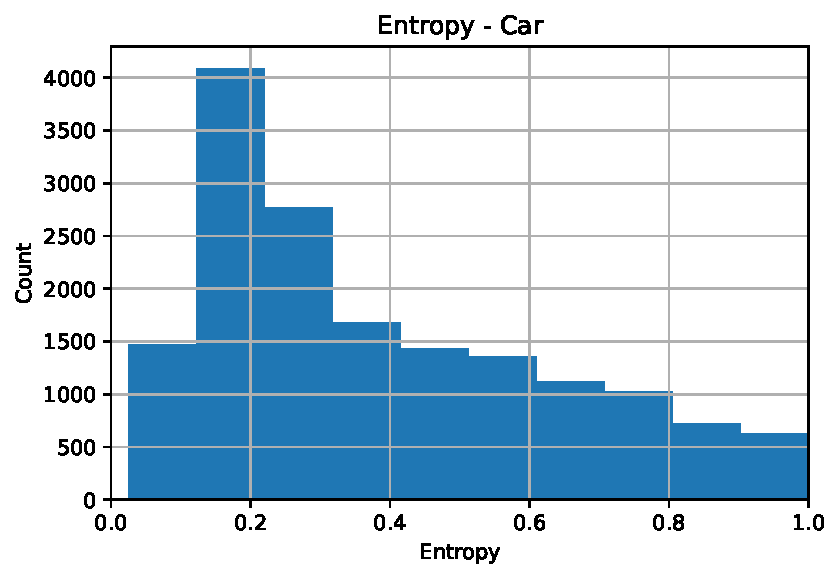
\includegraphics[scale = 0.4]{images/Part-Bayesian F_Pointnet_Results/Entropy_Car.pdf}
        \caption[Extracted frustum point cloud after Normalization]{Entropy for Car detection}
        \label{fig:Norm Point Cloud}
\end{figure}
\begin{figure}[!htbp]
        \centering
		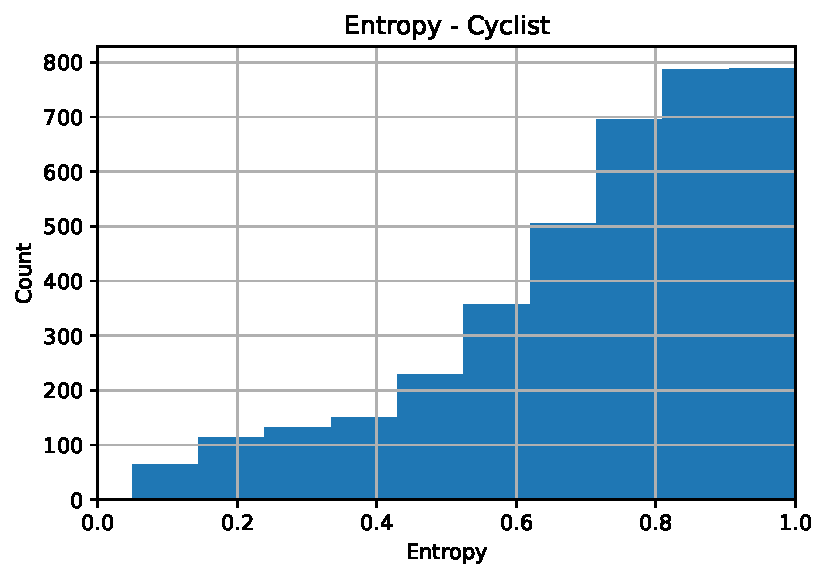
\includegraphics[scale = 0.4]{images/Part-Bayesian F_Pointnet_Results/Entropy_Cyclist.pdf}
        \caption[Extracted frustum point cloud after Normalization]{Entropy for Cyclist detection}
        \label{fig:Norm Point Cloud}
\end{figure}
\begin{figure}[!htbp]
        \centering
		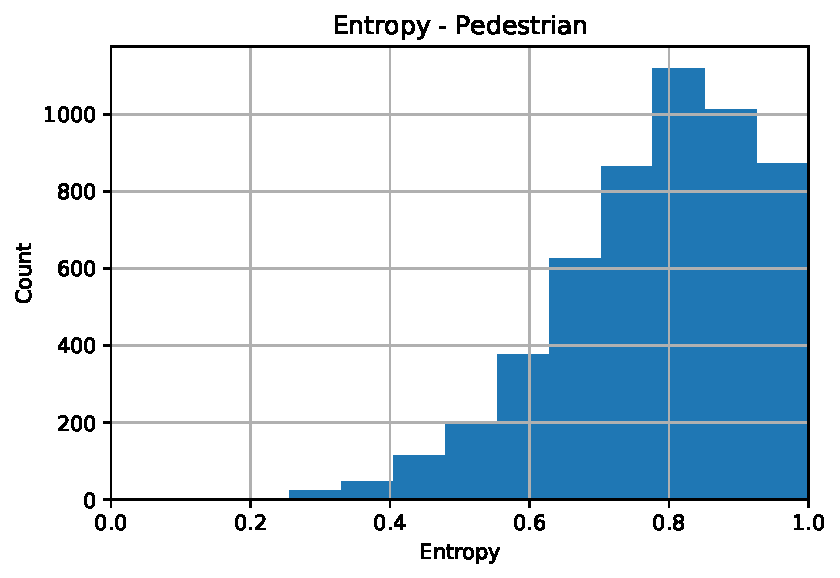
\includegraphics[scale = 0.4]{images/Part-Bayesian F_Pointnet_Results/Entropy_Pedestrian.pdf}
        \caption[Extracted frustum point cloud after Normalization]{Entropy for Pedestrian detection}
        \label{fig:Norm Point Cloud}
\end{figure}
\subsection{Visualizations}
\subsubsection{Uncertainty due to agents blocking one other}
The epistemic uncertainty of the car marked is high because of the car marked in green is blocking it in Image \ref{fig:Uncert_blockage-1}. Number of points available are very low in the bounding box, but the detection is made because of the bin size from the class in 2D object detection.
\begin{figure}[!htbp]
        \centering
		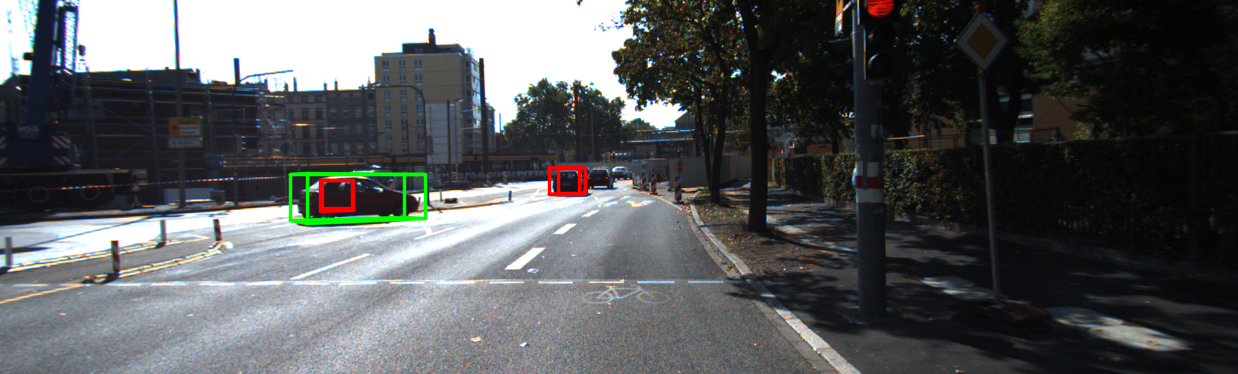
\includegraphics[width=75mm, scale = 0.4]{images/Uncertainty_results/3461_overlap_bbox.png}
        \caption[Extracted frustum point cloud after Normalization]{Predictions in the image plane.}
        \label{fig:Uncert_blockage-1}
\end{figure}
\begin{figure}[!htbp]
        \centering
		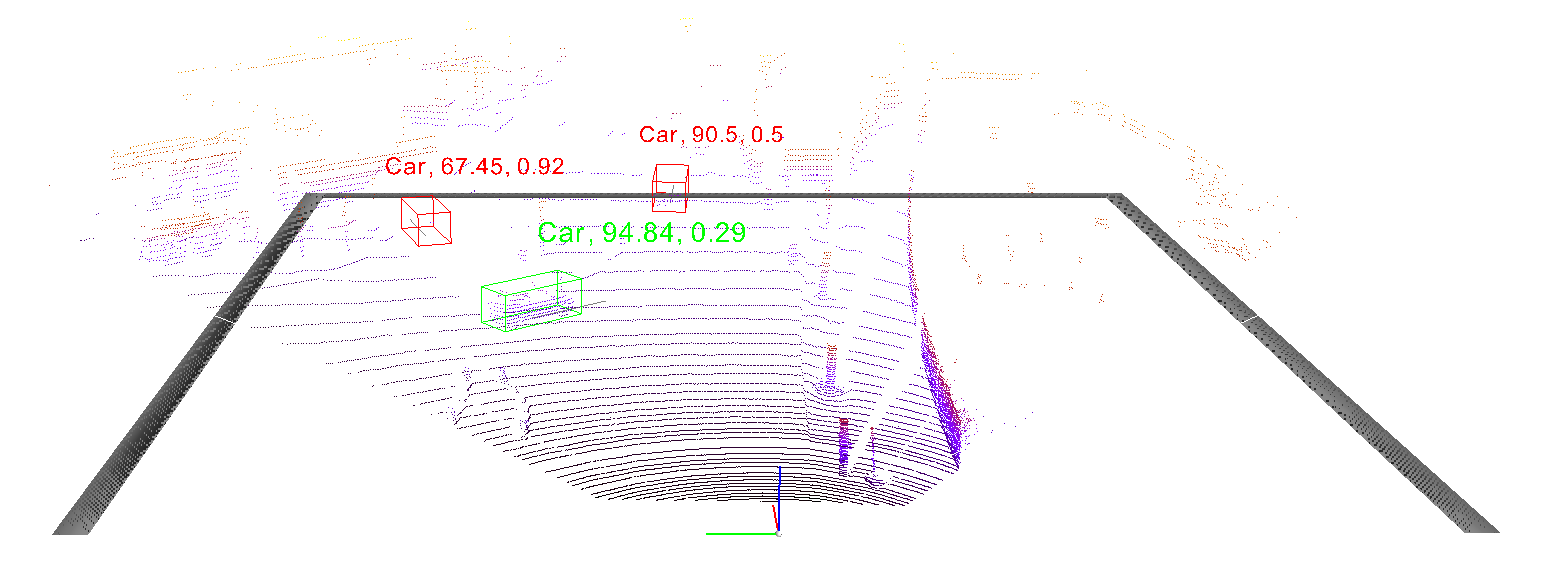
\includegraphics[width=75mm, scale = 0.4]{images/Uncertainty_results/3461_Follow_cam_view.png}
        \caption[Extracted frustum point cloud after Normalization]{Predictions in the LiDAR plane.}
        \label{fig:Uncert_blockage-1}
\end{figure}
\begin{figure}[!htbp]
        \centering
		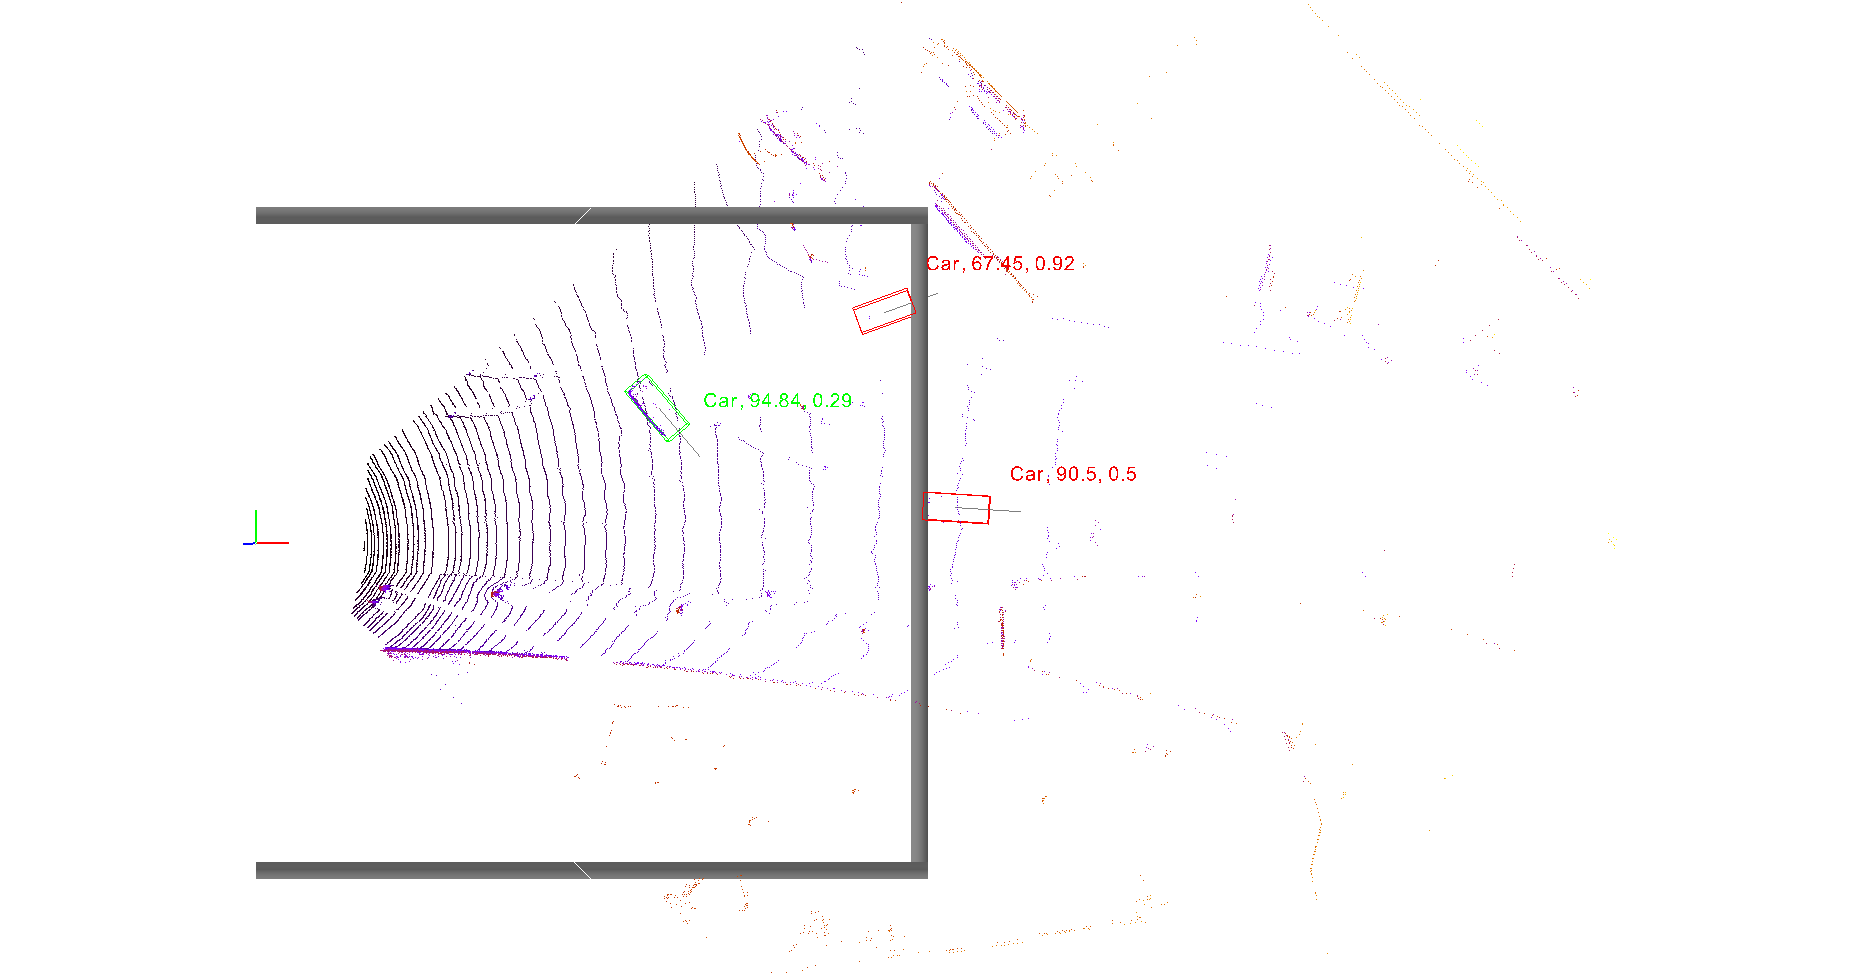
\includegraphics[width=75mm,scale = 0.4]{images/Uncertainty_results/3461_overlap.png}
        \caption[Extracted frustum point cloud after Normalization]{Predictions in the BEV projection of the LiDAR point cloud.}
        \label{fig:Uncert_blockage-1}
\end{figure}
\subsubsection{Epistemic uncertainty due to cluttered environments}
The epistemic uncertainty in a cluttered environment is high for every object present in the clutter. The total variance for every object as well is very high when compared to a non-cluttered scene. Because of the overlaps in the detection, the point cloud of one object is affecting the other underlying objects as well which results in high entropy outputs.
\begin{figure}[!htbp]
        \centering
		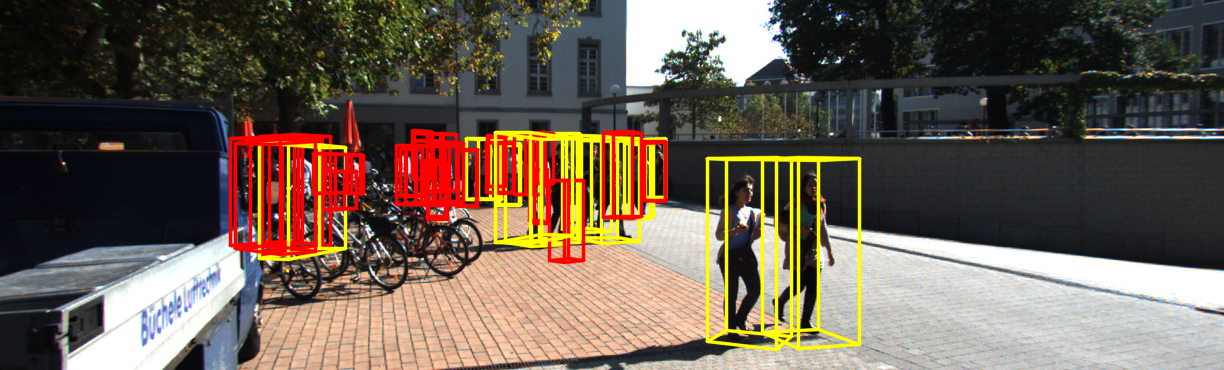
\includegraphics[width=75mm, scale = 0.4]{images/Uncertainty_results/5226_cluttered_bbox.png}
        \caption[Extracted frustum point cloud after Normalization]{Predictions in the image plane.}
        \label{fig:Uncert_blockage-1}
\end{figure}
\begin{figure}[!htbp]
        \centering
		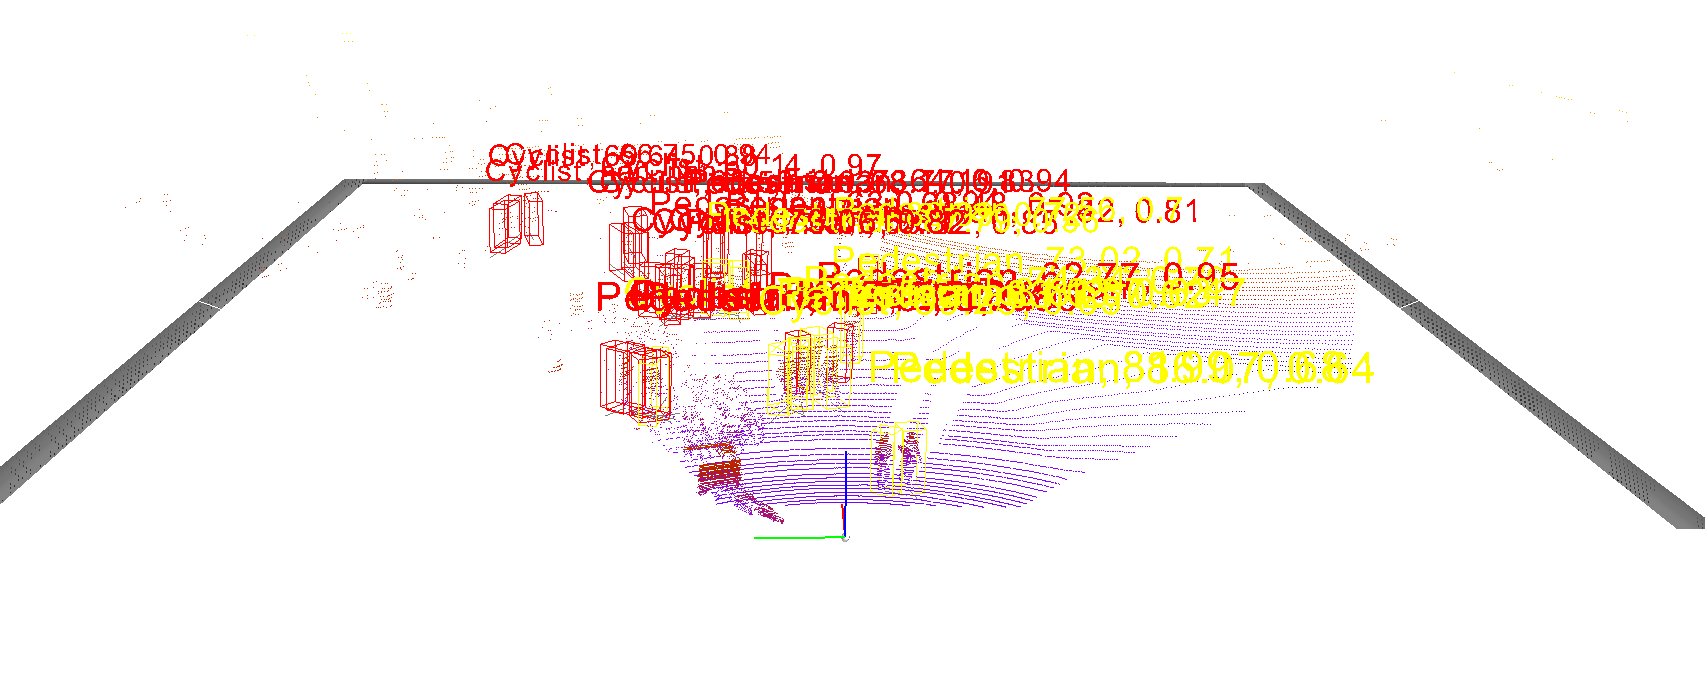
\includegraphics[width=75mm, scale = 0.4]{images/Uncertainty_results/5226_Follow_cam_view.png}
        \caption[Extracted frustum point cloud after Normalization]{Predictions in the LiDAR plane.}
        \label{fig:Uncert_blockage-1}
\end{figure}
\begin{figure}[!htbp]
        \centering
		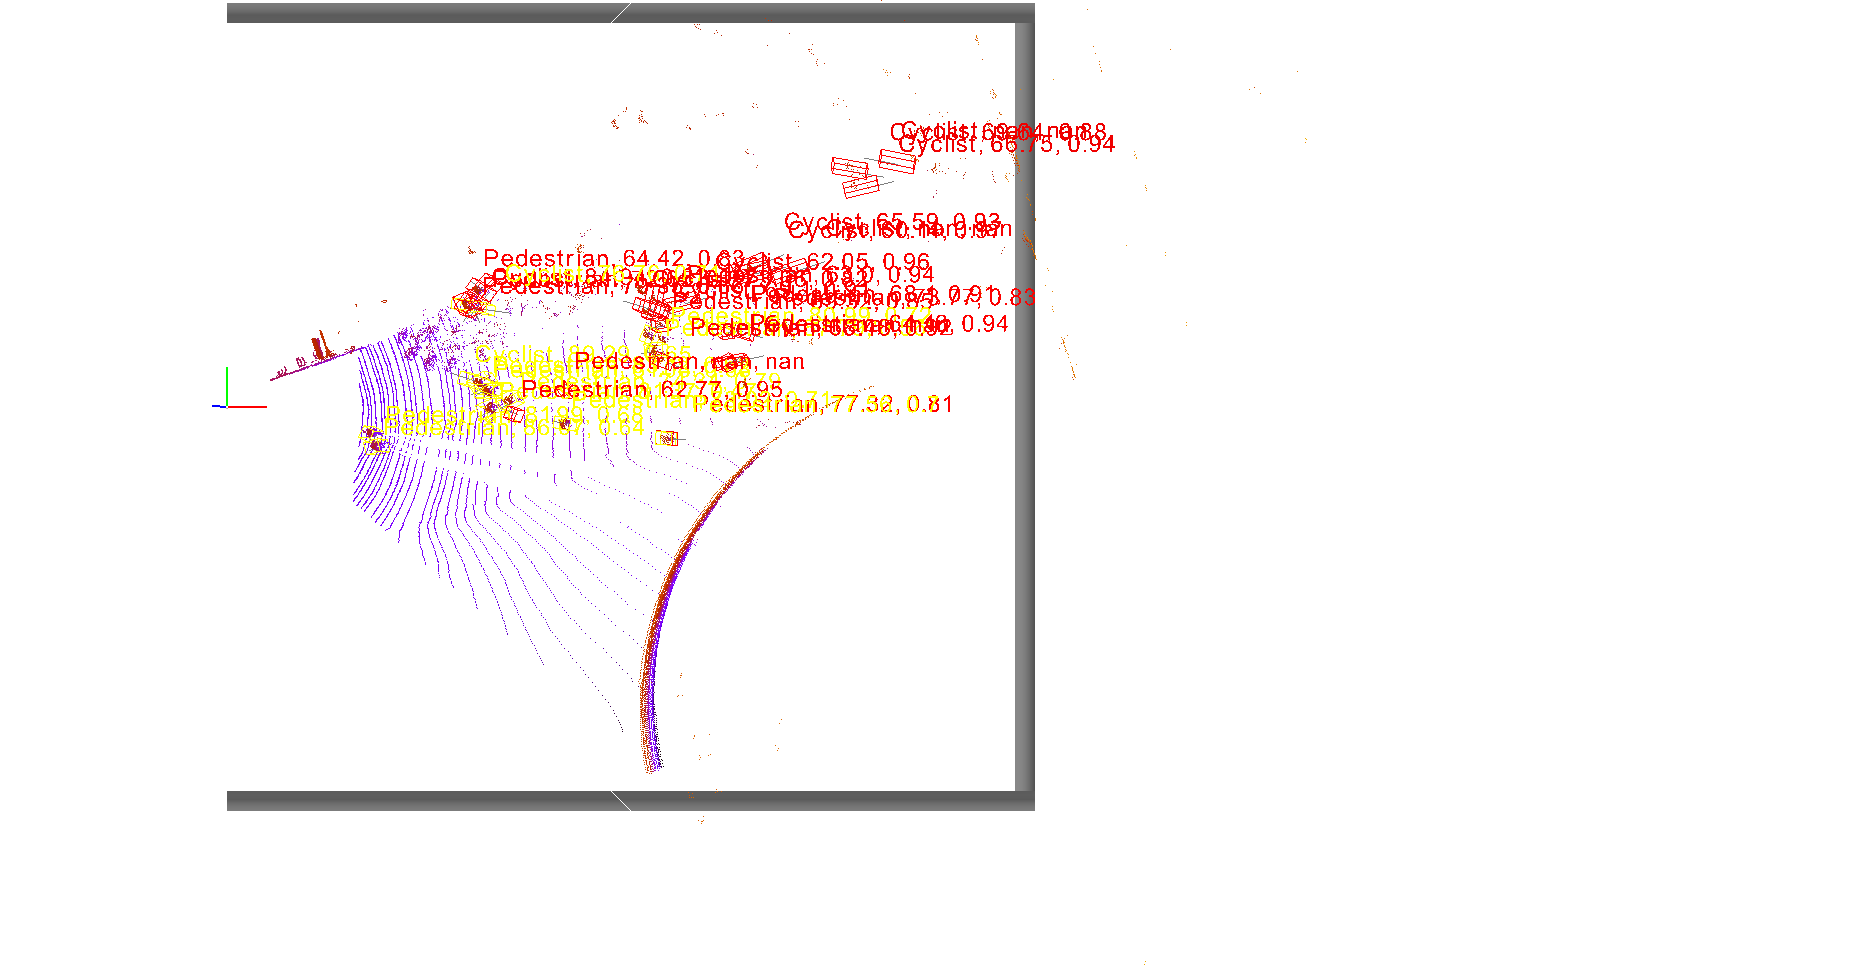
\includegraphics[width=75mm,scale = 0.4]{images/Uncertainty_results/5226_cluttered.png}
        \caption[Extracted frustum point cloud after Normalization]{Predictions in the BEV projection of the LiDAR point cloud.}
        \label{fig:Uncert_blockage-1}
\end{figure}
\subsubsection{Epistemic uncertainty due to distance to objects}
The epistemic uncertainty of the car marked in red is at a distance from the ego-vehicle which might result in:
        \begin{itemize}
            \item Reduced number of points in the extracted point cloud.
            \item Increased in the angle between centroid of the point cloud and the heading angle of the frustum point cloud, which might result in a overlapped bin size 
        \end{itemize}
\begin{figure}[!htbp]
        \centering
		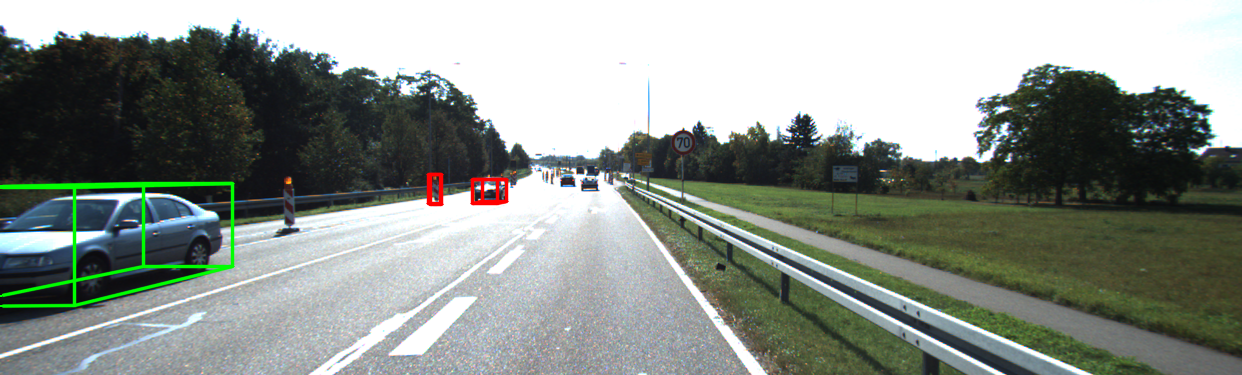
\includegraphics[width=75mm, scale = 0.4]{images/Uncertainty_results/3535_distance_-bbox.png}
        \caption[Extracted frustum point cloud after Normalization]{Predictions in the image plane.}
        \label{fig:Uncert_blockage-1}
\end{figure}
\begin{figure}[!htbp]
        \centering
		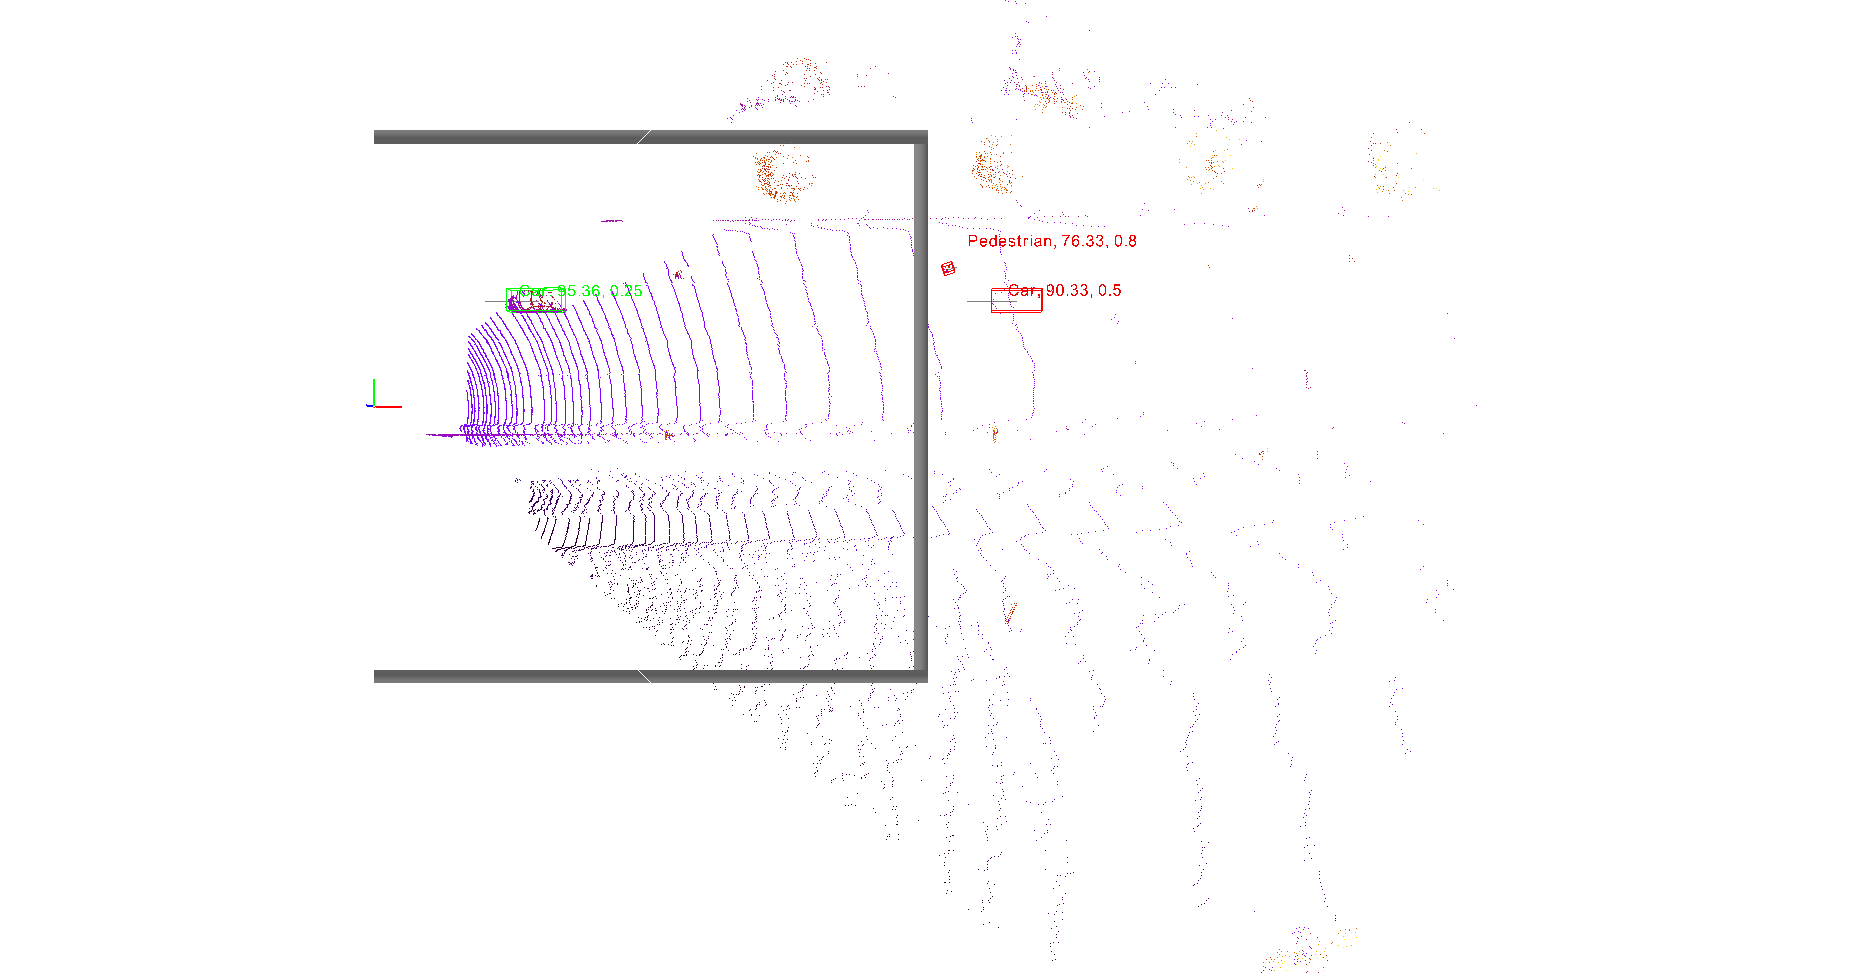
\includegraphics[width=75mm, scale = 0.4]{images/Uncertainty_results/3535_Follow_cam_view.png}
        \caption[Extracted frustum point cloud after Normalization]{Predictions in the LiDAR plane.}
        \label{fig:Uncert_blockage-1}
\end{figure}
\begin{figure}[!htbp]
        \centering
		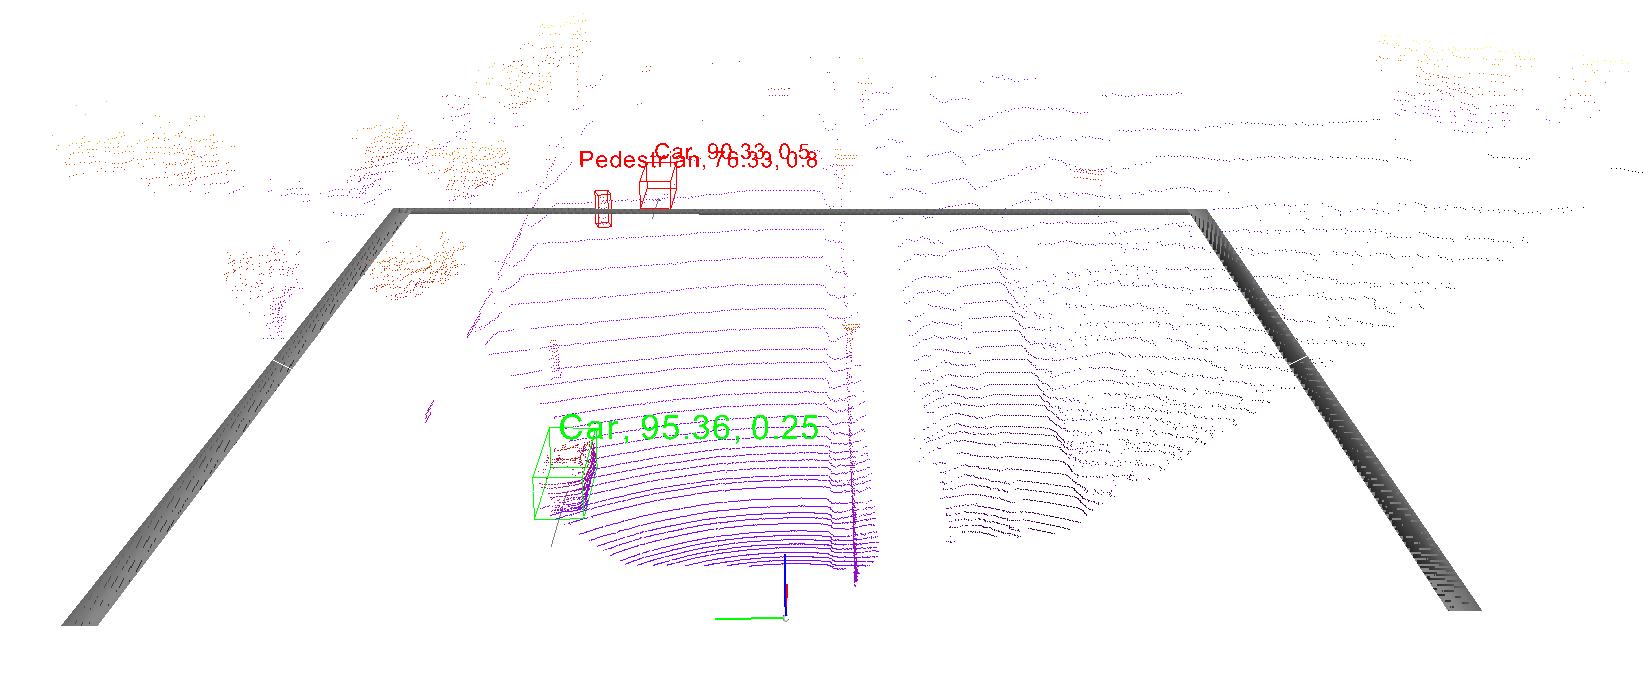
\includegraphics[width=75mm,scale = 0.4]{images/Uncertainty_results/3535_distance.png}
        \caption[Extracted frustum point cloud after Normalization]{Predictions in the BEV projection of the LiDAR point cloud.}
        \label{fig:Uncert_blockage-1}
\end{figure}
%-------------------------------------------------------------------------
\section{Conclusion and Future works}
In this paper we first train a point-wise Frustum-PointNet \cite{FPointnet2018} architecture to solve the 3-Dimensional (3D) object detection problem in the context of autonomous driving. The network is trained and tested on Lyft dataset \cite{Lyft2019}. We observed that the network performed on the same level as the network trained using KITTI dataset \cite{KITTI2012}. The comparison is done based on 3D Average-Precision values calculated using fixed limits set on Intersection-over-Union values.
    
Furthermore, we also modeled a Bayesian Neural Network based on the Frustum-PointNet \cite{FPointnet2018} to extract the uncertainty due to the weights. We concluded that the BNN performed better than the fixed-weight model.
% But, we observed that the difference in performance is not as expected. We believe that with the better tuning of the prior distribution placed on the weights, we can achieve better results.  ??

Further analysis on the extracted uncertainty showed that the point-wise model is over-confident. We visualized some samples which represented the model's over-confidence and confirm the need for the usage of uncertainty as a measure of confidence.


{\small
\bibliographystyle{ieee_fullname}
\bibliography{bibliography}
}

\end{document}
